\documentclass[report.tex]{subfiles}
\begin{document}
\subsection{Theoretical background}
When designing a pass- or stop-band filter, a low-pass filter is used as basis and then frequency shifted and impedance transformed. 

Theoretically designing a maximally flat 2\nd order lumped component band-pass filter using the parameters in table~\ref{table:filter specs} is done by first designing a low-pass filter with cut-off frequency equal to the desired center frequency ($\omega_c=\omega_0$). The center frequency is calculated from eq.~\ref{eqn:center frequency}.

\begin{equation}
    \omega_0 = \sqrt{\omega_U \cdot \omega_L} \approx 2.44~GHz
    \label{eqn:center frequency}
\end{equation}

A flat 2\nd order low-pass filter have the following filter constants (from table 5-2 in R. Ludwig).

\begin{equation*}
    g_0=g_3=1, g_1=g_2=1.4142
\end{equation*}

This low-pass filter can be realized with a series inductor and a shunt capacitor, both with a normalized value of $g_1~F$ and $g_2~H$ respectively. To convert this low-pass filter to a band-pass filter, Table 5-5 in R. Ludwig is considered. A series capacitor is appended to a series inductor, and a shunt capacitor is connected to an inductor in parallel (see fig.~\ref{fig:Filter A circuit}).

The new normalized values of the band-pass filter are calculated using eqs.~\ref{eqn:first filter value}-\ref{eqn:fourth filter value}.

\begin{equation}
    \label{eqn:first filter value}
    L_1=\frac{g_1}{\omega_U-\omega_L} \approx 
\end{equation}
\begin{equation}
    C_1=\frac{\omega_U-\omega_L}{\omega_0^2 g_1} \approx
\end{equation}
\begin{equation}
    L_2=\frac{\omega_U-\omega_L}{\omega_0^2 g_2} \approx
\end{equation}
\begin{equation}
    \label{eqn:fourth filter value}
    C_2=\frac{g_2}{\omega_U-\omega_L} \approx
\end{equation}

These normalized values can be de-normalized using eqn.~\ref{eqn:normalized inductance} and \ref{eqn:normalized capacitance} below

\begin{equation}
    \label{eqn:normalized inductance}
    \tilde{L_1}=L Z_0
\end{equation}
\begin{equation}
    \label{eqn:normalized capacitance}
    \tilde{C_2}=\frac{C}{Z_0}
\end{equation}

The normalized component values of the band-pass filter are summarized in table~\ref{table:filter values} and the final lumped circuit together with simulation setup and result is shown in fig.~\ref{fig:Filter A circuit} and \ref{fig:Filter A S-params}

\begin{table}[h]
    \centering
    \caption{Component values for a flat 2\nd order band-pass filter}
    \begin{tabular}{c | r @{.} l @{} l}
        Component & \multicolumn{2}{c}{Value} \\
        \hline
        $L_1$     & 140&7 & nH\\
        $C_1$     & 30&25 & fF\\
        $L_2$     & 75&6  & pH\\
        $C_2$     & 56&3  & pF\\
    \end{tabular}
    \label{table:filter values}
\end{table}

\clearpage
\begin{figure}[h]
    \centering
    \subfloat[Simulation setup] {
        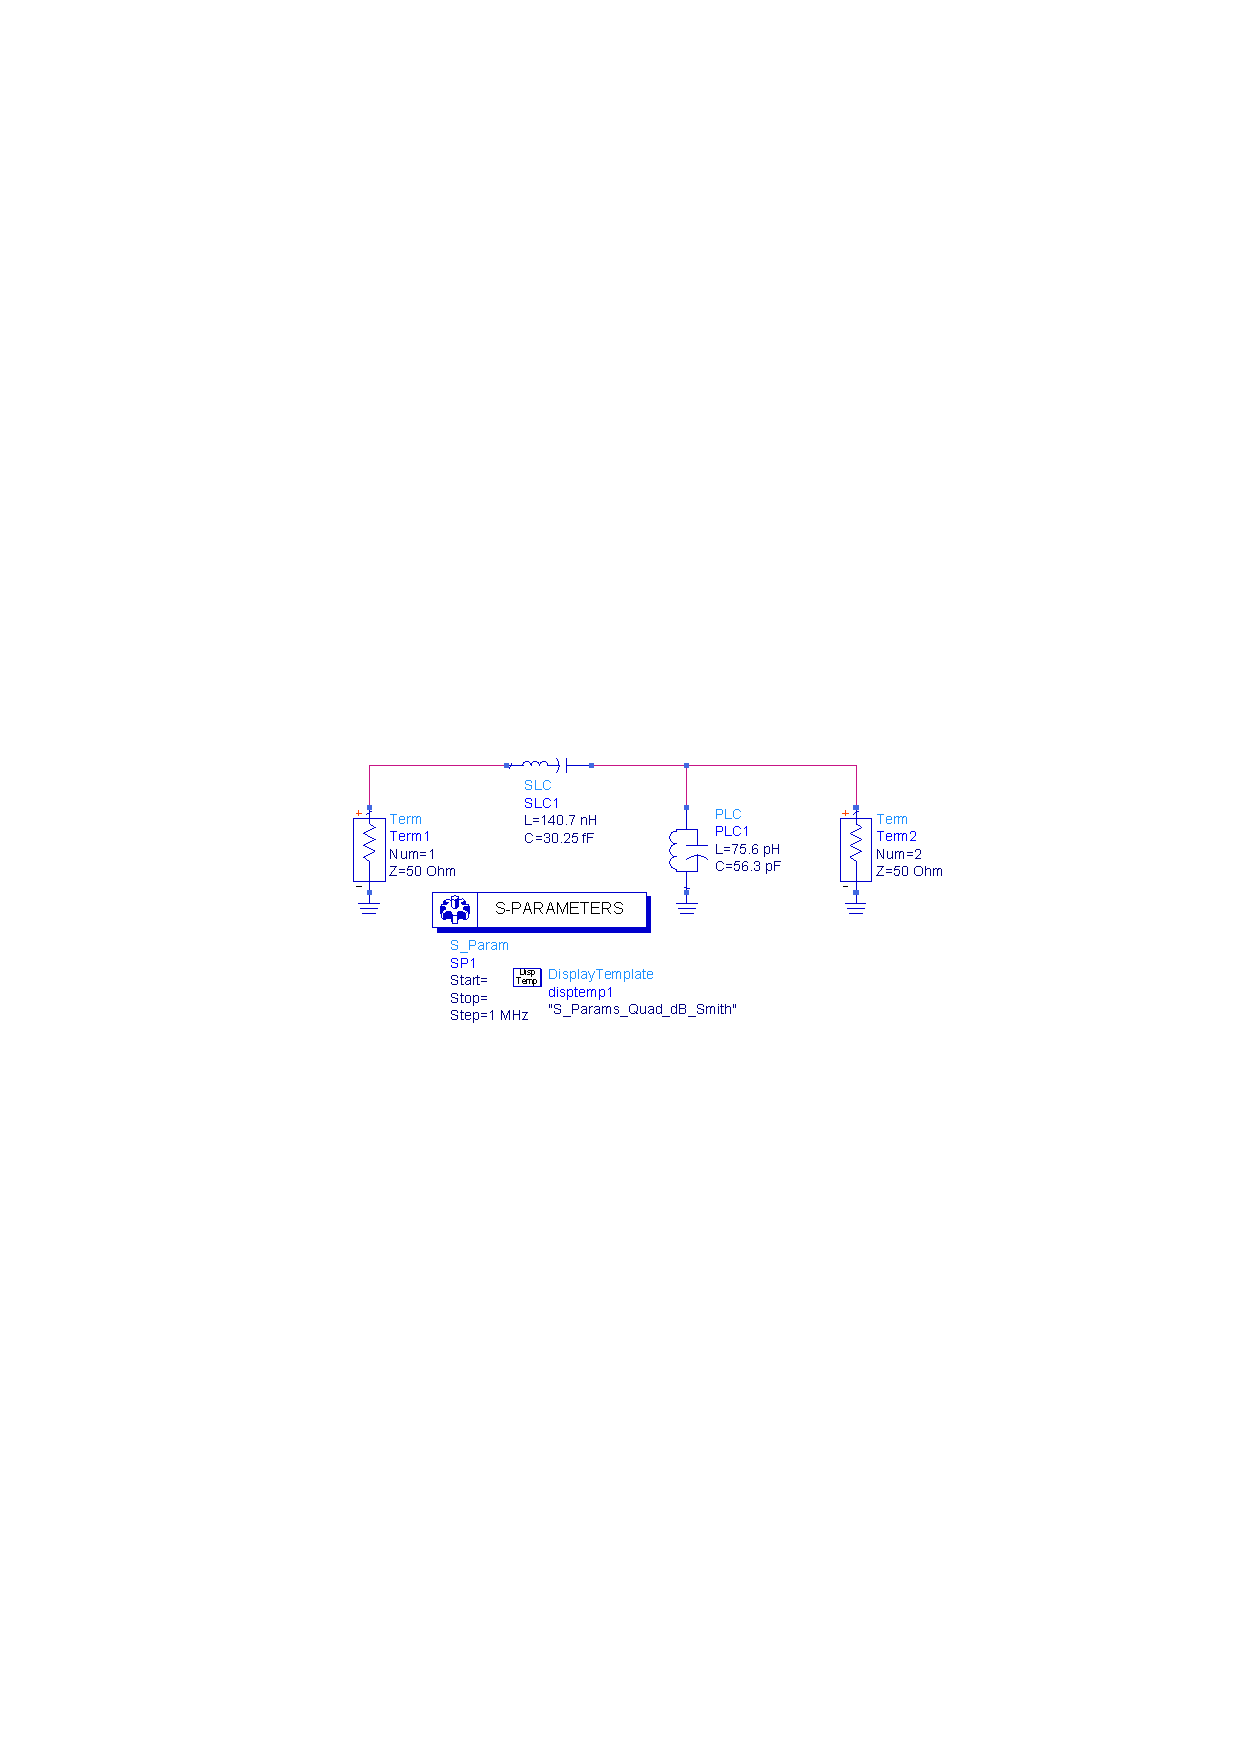
\includegraphics[width=0.8\linewidth]{filter_A_circuit}
        \label{fig:Filter A circuit}
    }
    
    \subfloat[S-parameters vs. frequency]{
        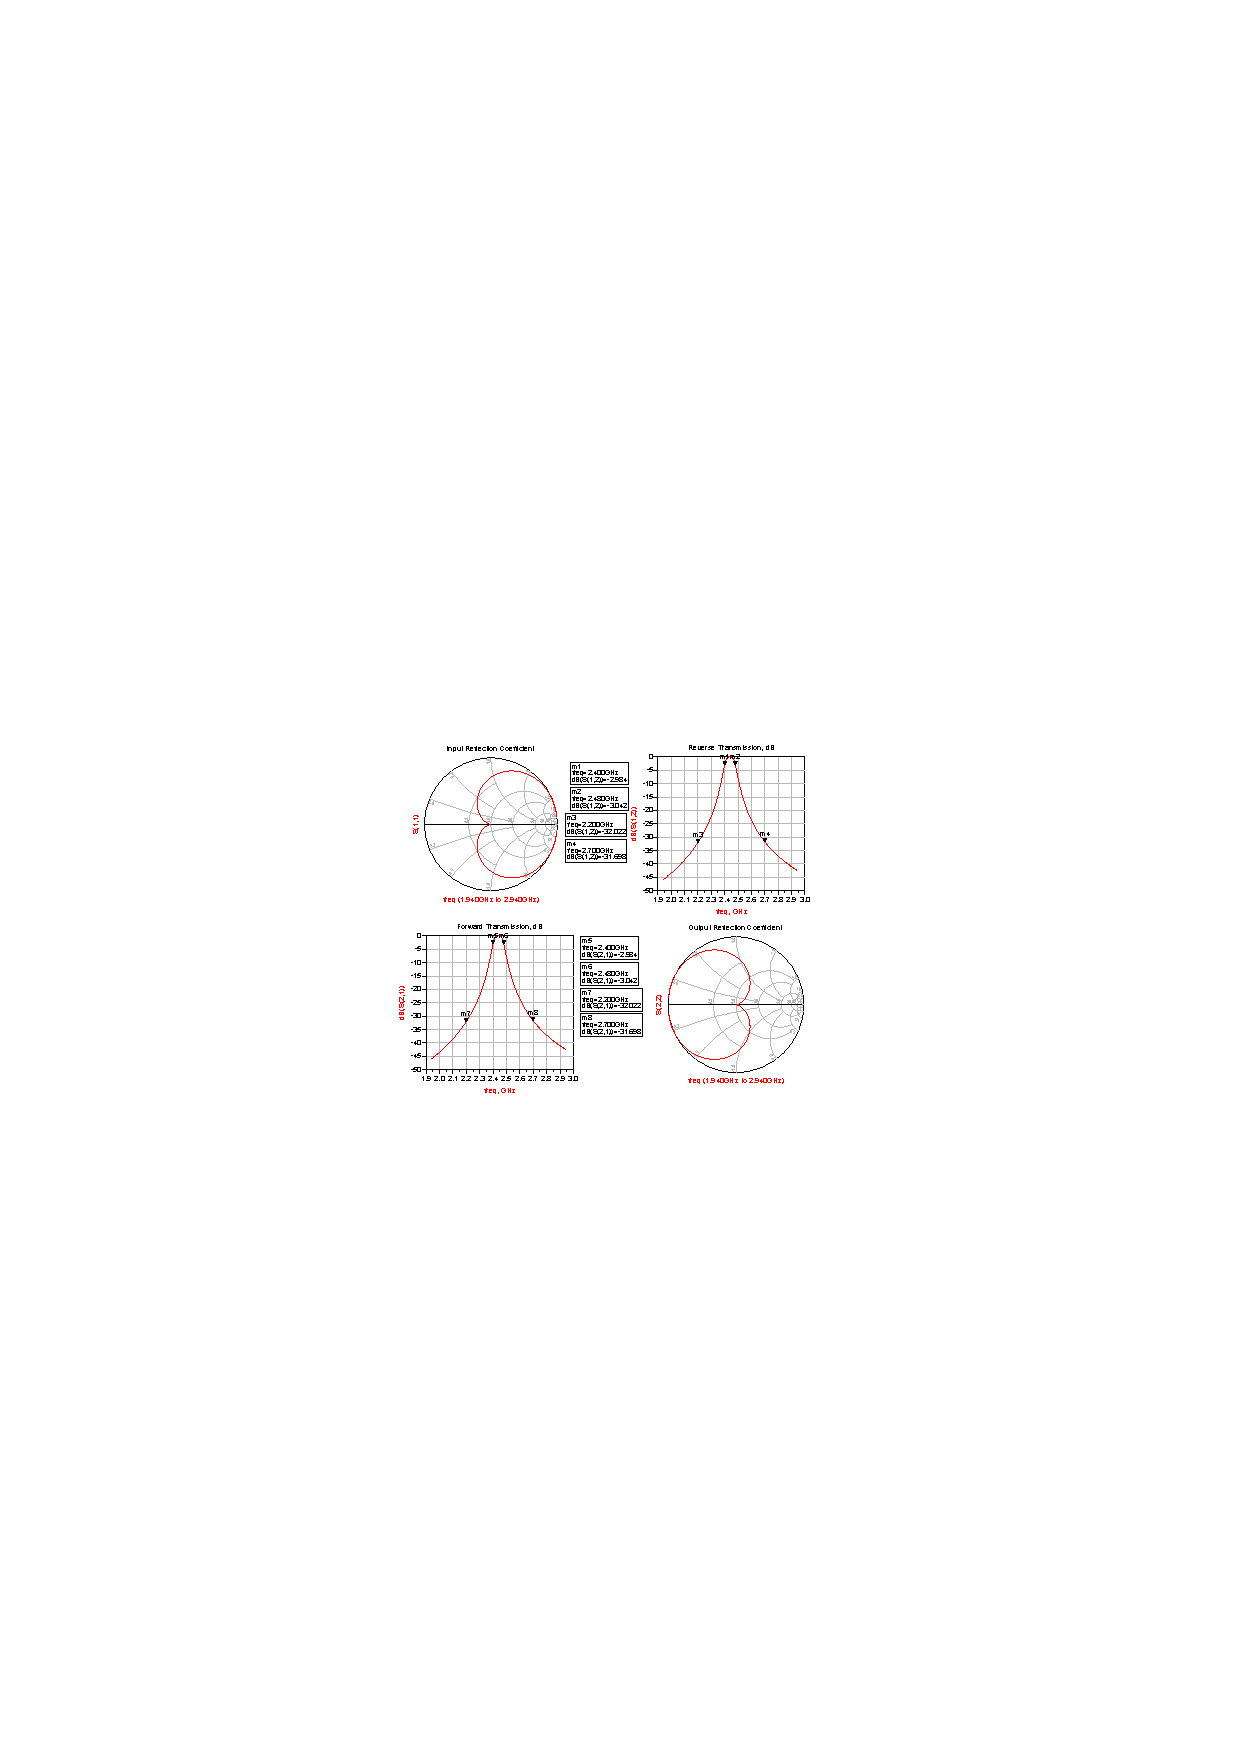
\includegraphics[width=0.8\linewidth]{S-params_filter_A}
        \label{fig:Filter A S-params}
    }
    \caption{Simulation setup and result of 2\nd order flat band-pass filter}
\end{figure}
\clearpage

\end{document}